\clearpage{\pagestyle{empty}\cleardoublepage}
\chapter{Strumenti utilizzati per la creazione dell'Infografica}               
\noindent In questo capitolo verranno illustrati tutti gli strumenti che verranno utilizzati per creare l'infografica finale. Verranno prima trattati gli aspetti di front-end come lo standard usato per le immagini ed il framework utilizzato per creare i vari layout. Successivamente verrà illustrato il funzionamento di React, il Framework Javascript utilizzato come base per l'applicazione. Infine verranno illustrate e descritte alcune librerie il cui uso ha reso il lavoro più semplice e veloce.
\section{Rappresentazione di immagini e Design responsivo}
\noindent Con design responsive si intende una tecnica di design che mira alla realizzazione di siti/blog in grado di adattarsi graficamente al dispositivo coi quali vengono visualizzati.
\noindent Il design responsivo è un tassello fondamentale per garantire una buona usabilità.\newline
Alcuni studi condotti in Italia dimostrano come su una audience totale di 30,7 milioni (circa il 56\% della popolazione), il 46,7\% accede ad internet da smartphone o dispositivi mobili mentre solo il 19,4\% effettua l'accesso da dispositivi desktop \cite{mobileFirst}.\newline
\subsection{Bootstrap}
\noindent Bootstrap è stato creato nel 2010, tramite Twitter, da @mdo and @fat.
\begin{figure}[H]
    \centering
    
\includegraphics[width=0.3\linewidth]{img/bootstrap-logo.png}
    \caption{Logo di Bootstrap \cite{bootstrap}.}
    \label{bootstrapLogo}
\end{figure}
\noindent È rapidamente diventato il framework più popolare per il front-end a livello mondiale.
Con le prime release della versione 2 vennero introdotti i primi fogli di stile (opzionali) per aggiungere funzionalità riguardanti il design responsive.\newline
Con l'uscita della versione 3 l'intera libreria è stata ripensata e riscritta per offrire supporto al design responsive con un approcio mobile-first.
La versione 4 di Bootstrap infine (quella attuale) ha subito due principali cambiamenti nella sua architettura:
\begin{itemize}
    \item una migrazione a Sass, un'estensione del linguaggio CSS che permette l'uso di variabili e di funzioni. L'estensione dei file Sass è .scss;
    \item l'uso di CSS flexbox, ovvero contenitori per elementi.
\end{itemize}

\noindent Bootstrap adotta un approcio mobile-first.
L'assunzione di base è che la maggior parte dei visitatori utilizzeranno uno smartphone a causa del sempre più crescente utilizzo di questo tipo di dispositivi.\newline
L'utilizzo continuo di media query è alla base di ogni layout creato utilizzando Bootstrap \cite{bootstrap}. \newline Moltissime classi offerte utilizzano i cosiddetti breakpoints. Si tratta di meccanismi che permettono di nascondere, mostrare o modificare il comportamento degli elementi a cui vengono applicate in base alla risoluzione dello schermo del visitatore.
Bootstrap mette a disposizione i seguenti breakpoints:
\begin{lstlisting}[language=CSS]
// Small devices (landscape phones, 576px and up) KEYWORD:sm
@media (min-width: 576px) { ... }

// Medium devices (tablets, 768px and up) KEYWORD:md
@media (min-width: 768px) { ... }

// Large devices (desktops, 992px and up) KEYWORD:lg
@media (min-width: 992px) { ... }

// Extra large devices (large desktops, 1200px and up) KEYWORD:xl
@media (min-width: 1200px) { ... } 
\end{lstlisting}
\noindent Segue un rapido esempio per l'uso dei breakpoints. Per la gestione dei margini e del padding Bootstrap mette a disposizione le classi di tipo \{property\}\{sides\}-\{breakpoint\}-\{size\}.
\begin{itemize}
    \item \textbf{\{property\}}: \textbf{m} se si vuole aggiungere un margine, \textbf{p} se si vuole aggiungere del padding;
    \item \textbf{{\{sides\}}}: \textbf{t} per top, \textbf{b} per bottom, \textbf{r} per right, \textbf{l} per left, \textbf{x} per right e left, \textbf{y} per top e bottom;
    \item \textbf{\{breakpoints\}}: se omesso, la classe funziona su qualsiasi tipo di schermo, anche i più piccoli, altrimenti funziona solo sugli schermi più grandi anche solo di un pixel del breakpoint specificato;
    \item \textbf{\{size\}}: Bootstrap non utilizza valori statici per specificare di quanto deve essere il padding o il margin. Il valore che può assumere size va da 0 a 5, e sono valori che indicano quando deve essere grande il moliplicatore che gestisce lo spazio. 0 significa nessun padding/margin.
    
\end{itemize}
\noindent Se si desidera applicare un piccolo margine a destra ad un determinato elemento solo se il visitatore lo visualizza su uno schermo con larghezza maggiore di 992px, le classi che l'elemento dovrà assumere saranno \textbf{mr-0 mr-lg-2}.\newline
\textbf{mr-0} significa nessun margine a destra su qualsiasi tipo di schermo. \textbf{mr-lg-2} invece vuol dire margine a destra con proporzione 2 solo su schermi più grandi di 992px. Combinando insieme le due classi otteniamo un margine solo su schermi con larghezza maggiore di 992px \cite{bootstrapDoc}.



\subsection{Scalable Vector Graphics}
\noindent Scalable Vector Graphics (SVG) è un linguaggio di markup usato per la rappresentazione di immagini a due dimensioni creato e mantenuto da W3C.\newline
SVG è supportato da tutti i browser moderni sia in versione desktop che mobile, anche se non tutte le funzionalità sono completamente compatibili.\newline
Attualmente, una nuova versione di SVG denominata SVG2 è in fase di sviluppo. SVG2 punta a migliorare la propria integrazione con HTML, CSS, DOM, oltre a deprecare molte funzionalità non supportate dalla totalità dei browser.
SVG permette di trattare tre tipi di oggetti grafici:
\begin{itemize}
    \item forme geometriche create attraverso l'uso di rette e curve;
    \item immagini della grafica raster ovvero immagini digitali, fortemente in contrapposizione con la grafica di tipo vettoriale che offre SVG;
    \item testo, eventualmente anche cliccabile.
\end{itemize}
Una buona parte dei software grafici sono in grado di esportare grafiche anche in formato SVG.\newline
\textbf{Perché utilizzare SVG?}\newline
Le potenzialità di SVG sono degne di attenzione, in quanto si basano sulla grafica vettoriale scalabile:
\begin{itemize}
    \item ogni elemento grafico è definito matematicamente utilizzando termini vettoriali anziché usando una griglia di pixel;
    \item la qualità dell'immagine viene mantenuta a qualsiasi ridimensionamento. Non vi sono effettivamente particolari trasformazioni sulle immagini da eseguire per il rimpicciolimento o l'ingrandimento. La qualità della visualizzazione dell'immagine è sempre massima.
\end{itemize}

\begin{figure}[H]
    \centering
    
\includegraphics[width=0.45\linewidth]{img/rastVect.png}
    \caption{Differenze tra un'immagine Bitmap e un'immagine Vettoriale \cite{wikipediaSVG}.}
    \label{rastVect}
\end{figure}

\noindent Ci sono anche svantaggi nell'utilizzo di SVG. Per garantire sempre la qualità massima il calcolatore deve renderizzare l'immagine ogni volta che avviene un ridimensionamento. L'uso di SVG potrebbe dunque causare un maggior dispendio di risorse \cite{svgOfficial}.
\section{React, il Framework per le interfacce utente}
\noindent React \cite{reactPage} è una libreria Javascript utilizzata per creare interfacce utente.\newline Creata e mantenuta 
principalmente da Facebook, è molto utile per la creazione di componenti separabili e quindi riutilizzabili in più pagine.\newline

\begin{figure}[H]
    \centering
    
\includegraphics[width=0.3\linewidth]{img/react.png}
    \caption{Logo di React \cite{reactImg}.}
    \label{reactLogo}
\end{figure}
\subsection{Conoscenze pregresse necessarie}
\noindent I Framework sono spesso basati su linguaggi già esistenti e si occupano di semplificarli creando nuovi meccanismi.\newline
React non introduce alcun tipo di novità per quanto riguarda il front-end.
L'HTML (HyperText Markup Language) rimane lo standard per quanto riguarda la creazione della struttura delle pagine. \newline
CSS (Cascading Style Sheets) è invece il linguaggio utilizzato per la formattazione dei documenti.\newline
Javascript è il linguagggio orientato agli oggetti e agli eventi, utilizzato nella programmazione Web lato client su cui è basato React. Qualsiasi funzione o meccanismo di Javascript funziona perfettamente anche su un'applicazione React.\newline
Sono stati utilizzati per la creazione dell'infografica anche altri strumenti più specifici, come Sass (Syntactically Awesome StyleSheets) \cite{sass}, un'estensione del linguaggio CSS e TypeScript \cite{typescript}, un linguaggio di programmazione sviluppato da Microsoft. Per utilizzare React non è comunque necessario conoscere queste due tecnologie.\newline
Il Json (JavaScript Object Notation) è il formato utilizzato per il salvataggio in locale degli oggetti, oltre allo standard adottato per le comunicazioni client/server.

\subsection{Introduzione a Node.js}
\noindent Node.js \cite{nodejs} è una runtime di JavaScript multipiattaforma per l'esecuzione di codice JavaScript, costruita sul motore JavaScript V8 di Google Chrome.\newline
Node.js dispone di una grande quantità di moduli scritti completamente in Javascript.
Essendo il progetto open source è inoltre possibile per gli sviluppatori aggiungere i propri moduli in modo da renderli disponibili pubblicamente \cite{nodejs}.\newline 
\noindent Il gestore di pacchetti predefinito per l'ambiente di runtime JavaScript Node.js si chiama Node Package Manager (npm).
npm può essere richiamato tramite linea di comando usando la seguente sintassi:
\begin{verbatim}
    npm <command> [args]
\end{verbatim}
Il comando base per ottenere un pacchetto è:
\begin{verbatim}
    npm install packet_name
\end{verbatim}
Tutte le dipendenze e i conflitti vengono gestiti automaticamente \cite{npmDoc}.
\newline Grazie a Node.js è possibile creare un progetto React utilizzando il comando seguente:
\begin{verbatim}
    npx create-react-app project
\end{verbatim}
\textbf{npx} è uno strumento integrato in npm in grado di eseguire pacchetti, anche se non sono ancora installati nel sistema.\newline
Sarà poi possibile avviare il server di sviluppo usando i seguenti comandi:
\begin{verbatim}
    cd project
    npm start
\end{verbatim}
L'interfaccia sarà poi visualizzabile all'indirizzo \texttt{http://localhost:3000} \cite{reactGetStart}.
 
\subsection{Principi base di React}
\label{sub:princReact}
\noindent React utilizza un approccio dichiarativo simile all’HTML, per definire i componenti che rappresentano l’interfaccia.\newline
Sebbene non sia obbligatorio, React raccomanda l'utilizzo di JSX, un'estensione sintattica di Javascript.\newline
Dopo la compilazione, le espressioni JSX diventano normali chiamate a funzioni che producono oggetti JavaScript. È possibile in JSX assegnare il contentuto di una costante (o di una variabile) come segue:
\begin{lstlisting}[language=Javascript]
    const element = <h1> Hello, world! </h1>;
\end{lstlisting}
Grazie a JSX è possibile suddividere il codice su più linee per renderlo più leggibile.
\begin{lstlisting}[language=Javascript]
    const name = 'Giuseppe Verdi';
    const element = <h1>Hello, {name}</h1>;
    ReactDOM.render(
     element,
     document.getElementById('root')
    );
\end{lstlisting}

\noindent React è uno strumento si occupa di dividere la struttura dell'interfaccia in sottoparti in modo che siano più semplici da gestire.\newline
La figura \ref{reactMock} rappresenta un esempio di UI che si desidera creare utilizzando React.
\begin{figure}[H]
    \centering
    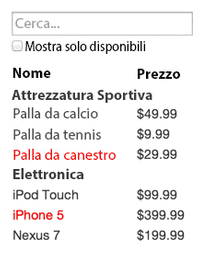
\includegraphics[width=0.4\linewidth]{img/thinking-in-react-mock.png}
    \caption{Mockup di una UI \cite{reactGetStart}.}
    \label{reactMock}
\end{figure}
\noindent Invece di separare struttura e logica, React preferisce non dividere le responsabilità.
\newline Vengono infatti utilizzati i Componenti, unità spesso collegate tra loro con il solo principio di composizione, i quali contengono sia la loro struttura sia la logica di singoli elementi della pagina.
La suddivisione in componenti dell'UI in figura \ref{reactMock} può avvenire come riportato in figura \ref{reactComp}.

\begin{figure}[H]
    \centering
    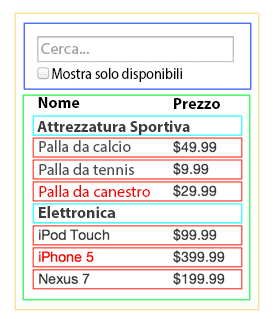
\includegraphics[width=0.40\linewidth]{img/thinking-in-react-components.png}
    \caption{Suddivisione in componenti della UI \cite{reactGetStart}.}
    \label{reactComp}
\end{figure}

Analizziamo la suddivisione effettuata partendo dagli elementi più interni:
\begin{itemize}
    \item \textbf{Rosso}: rappresenta un elemento di una lista. Contiene solo due stringhe: il nome e il prezzo dell'oggetto;
    \item  \textbf{Azzurro}: rappresenta il nome di una determinata lista. Contiene solo una stringa: il titolo;
    \item  \textbf{Verde}: è il componente contenitore di tutte le liste;
    \item \textbf{Blu}: rappresenta il filtro dell'interfaccia, contiene solo una textbox e una checkbox. Importante notare che è l'unico componente con cui l'utente può interagire;
    \item  \textbf{Arancione}: Contenitore dell'UI.
\end{itemize}
La struttura dell'UI è quindi suddivisibile in componenti.
Una volta identificati, i componenti vanno ordinati gerarchicamente. La UI è quindi rappresentabile nel seguente modo:
\renewcommand\labelitemii{$\bullet$}
\renewcommand\labelitemiii{$\bullet$}
\begin{itemize}
    \item TabellaProdottiRicercabile
    \begin{itemize}
        \item BarraRicerca
        \item TabellaProdotti
        \begin{itemize}
            \item RigaCategoriaProdotti
            \item RigaProdotto
        \end{itemize}
    \end{itemize}
\end{itemize}
\noindent Potrebbe capitare che la logica non si trovi necessariamente in ogni componente.
Esistono infatti componenti che si comportano da contenitori per altri componenti.
Proprio questi ultimi potrebbero contenere la logica dei loro figli e gestirli ad un livello più alto, per esempio perché si desidera che interagiscano a loro volta con altri componenti che altrimenti non potrebbero raggiungere.\newline
Nell'esempio l'utente può interagire solo col componente ``BarraRicerca" che però non può contenere la logica perché l'iterazione avviene con elementi interni a ``TabellaProdotti" che si trova sullo stesso livello gerarchico.\newline
In questo caso, tutta la logica è infatti contenuta in ``TabellaProdottiRicercabile" che può accedere ad entrambi i componenti \cite{thinkReact}.\newline
Quando due o più componenti devono interagire tra loro è infatti sempre il componente proprietario comune a gestire tutta la logica \cite{reactGetStart}.\newline


\noindent Il componente RigaProdotto si occupa di mostarre le informazioni dei singoli elementi della lista. Esiste un solo sorgente per il componente RigaProdotto che prende in input dei parametri, più precisamente una proprietà ``nome" e una ``prezzo". In React questi parametri di ingresso prendono il nome di \textit{props}. Un componente di tipo RigaProdotto può essere istanziato nel seguente modo:
\begin{lstlisting}[language=HTML5]
    <RigaProdotto nome={"Palla da calcio"} prezzo={49.99}/>
\end{lstlisting}
Mentre all'interno del componente l'informazione è reperibile tramite la parola chiave \textit{this}:
\begin{lstlisting}[language=html]
    <tr>
        <td>{this.props.nome}</td>
        <td>${this.props.prezzo}</td>
    </tr>
\end{lstlisting}
Oltre alle props un componente può anche avere uno stato interno.
Lo \textit{state} è simile alle props ma è privato e completamente controllato dal componente in cui è racchiuso.
Per inizializzare uno stato all'interno di un componente è necessario farlo nel costruttore.
\begin{lstlisting}[language=Javascript]
  constructor(props) {
    super(props);
    this.state = {checked: false};
  }
\end{lstlisting}
È possibile modificare lo stato tramite l'apposita funzione setter.
\begin{lstlisting}[language=Javascript]
    this.setState({
          checked: true
    });
\end{lstlisting}
È proprio grazie agli stati che possiamo gestire la logica interna della nostra applicazione.\newline
Nell'esempio, utilizzando una funzione Javascript si possono facilmente nascondere elementi da una lista facendo il controllo sullo stato che cambia il suo valore in base agli input dell'utente.
\section{Librerie aggiuntive}   
\noindent In questa sezione verranno trattate librerie aggiuntive per la manipolazione e la creazione di immagini SVG e per le animazioni di elementi sul DOM. Oltre a descrivere le librerie verranno anche illustrate le modalità usate per l'importazione in un ambiente basato su React.

\subsection{Animazioni con Anime.js}
\noindent Anime.js è una libreria Javascript usata per gestire le animazioni delle pagine.\newline
La sintassi usata è proprietaria, ma è possibile utilizzare selettori CSS per scegliere quali elementi animare.
Sono inoltre disponibili tutte le funzioni CSS relative alle animazioni, per esempio il seguente codice:
\begin{lstlisting}[language=Javascript]
    anime({
        targets: '.el',
        translateX: 250
    });
\end{lstlisting}
si occupa di traslare di 250 pixel verso destra (lungo l'asse delle X) gli elementi denotati con classe "el".
\begin{figure}[H]
\centering
\begin{minipage}{.5\textwidth}
  \centering
  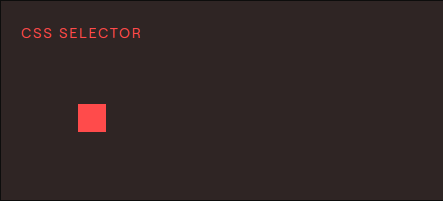
\includegraphics[width=.9\linewidth]{img/beforeAnime.png}
  \captionof{figure}{Elemento prima \\dell'animazione \cite{animeDoc}.}
\end{minipage}%
\begin{minipage}{.5\textwidth}
  \centering
  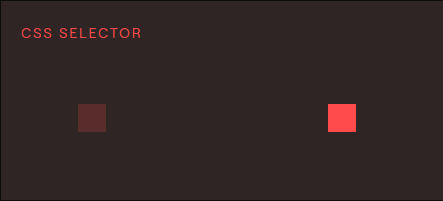
\includegraphics[width=.9\linewidth]{img/afterAnime.png}
  \captionof{figure}{Elemento dopo \\l'animazione \cite{animeDoc}.}
\end{minipage}
\end{figure}
\noindent Anime.js \cite{animejs} è una libreria Javascript, ne consegue che il suo funzionamento è stato pensato per applicazioni Javascript pure.\newline
Non è possibile utilizzare la versione di Anime.js fornita sul sito ufficiale, in quanto va in conflitto con il modo di gestire la logica di React, in particolare non è possibile usare Anime.js insieme a JSX.
Per inserire la libreria all'interno del progetto, il comando da utilizzare non è: \begin{verbatim}
    npm install animejs
\end{verbatim} come consigliato sul sito ufficiale, ma: \begin{verbatim}
    npm install react-animejs
\end{verbatim}
ReactAnime è un wrapper di Anime.js, che permette l'uso della libreria anche su progetti basati su React.
La sintassi è ovviamente leggermente diversa da quella originale, ma il funzionamento resta il medesimo.\newline
Su ReactAnime, il codice illustrato poco sopra muta in:
\begin{lstlisting}[language=HTML5]
    <Anime initial={[{
        targets: ".el",
        translateX: 250
     }]}>
        <div className="el"> [...] </div>
    </Anime>
\end{lstlisting}
La documentazione del sito ufficiale rimane completamente affidabile ed è possibile seguirla senza problemi.
\subsection{Creazione di immagini con Snap.svg}
\noindent Snap.svg \cite{snapSite} è una libreria improntata alla manipolazione e alla creazione di immagini SVG.\newline
\begin{figure}[H]
\centering
\begin{minipage}{.5\textwidth}
  \centering
  
\includegraphics[width=.54\linewidth]{img/snap.png}
  \captionof{figure}{Logo di Snap.svg \cite{snapSite}.}
\end{minipage}%
\begin{minipage}{.5\textwidth}
  \centering
  
\includegraphics[width=.9\linewidth]{img/snap2.jpg}
  \captionof{figure}{Mascotte di Snap.svg \cite{snapSite}.}
\end{minipage}
\end{figure}
\noindent Ricordiamo che l'importazione standard delle immagini usata da React preserva la scalabilità al variare della risoluzione.\newline
Snap.svg si rivela molto utile soprattuto per la creazione rapida di elementi SVG nel DOM.
Per creare un cerchio all'interno del contenitore con id ``container" la sintassi da usare è la seguente:
\begin{lstlisting}[language=JavaScript]
    var s = Snap("#container");
    var bigCircle = s.circle(150, 150, 100);
\end{lstlisting}
I valori numerici sono rispettivamente le coordinate x e y del cerchio e il suo raggio.
È possibile  aggiungere proprietà al cerchio appena creato:
\begin{lstlisting}[language=JavaScript]
    bigCircle.attr({
        fill: "#bada55",
        stroke: "#000",
        strokeWidth: 5
    });
\end{lstlisting}
Il risultato è rappresentato in figura \ref{fig:snapCircle}.
\begin{figure}[H]
    \centering
    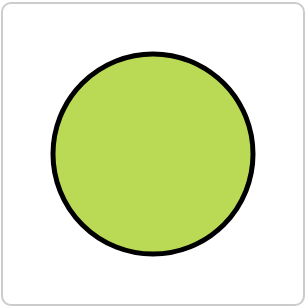
\includegraphics[width=0.45\linewidth]{img/snapCircle.png}
    \caption{Cerchio creato utilizzando SnapSVG \cite{snapSite}.}
    \label{fig:snapCircle}
\end{figure}

\noindent Anche Snap.svg, proprio come Anime.js non è però facilmente importabile in React.\newline
È necessario usare la versione wrapper che su npm prende il nome di snapsvg-cjs.
Il comando da eseguire per ottenere il pacchetto è:
\begin{verbatim}
    npm install snapsvg-cjs
\end{verbatim}
La sintassi non differisce troppo dalla versione base di Snap.svg